\documentclass{article}
\usepackage[utf8]{inputenc}
\usepackage{graphicx}
\title{Series de Tiempo en Pitiquito, Sonora}
\author{Mario Antonio Martínez Cerda}
\date{15 de enero de 2021}

\begin{document}
\maketitle
\section{Introducción.}

Durante el siguiente documento, veremos un análisis climatológico de la ciudad de Pitiquito, Sonora. Intentando observar los cambios que han sucedido en el clima y su comportamiento desde el año 1952 hasta 2015. Una de las herramientas que utilizaremos para facilitar el análisis de los cambios con el tiempo, serán las gráficas publicadas por la CONAGUA.
\maketitle

\section{Desarrollo.}
\subsection{Generalidades}
Pitiquito es un municipio del estado mexicano de Sonora, ubicada al norte de su territorio. Fundada en 1695 por el padre Eusebio Francisco Kino, con una población total de 9236 habitantes (datos de 2010). Cuenta con una latitud de 030°698', longitud de -112°100' y una altitud de 284 msnm.\\\\El clima del municipio es de tipo seco semicálido, teniendo una temperatura media máxima mensual de 31.4°C en los meses de julio y agosto, mientras que, en los meses de diciembre y enero obtiene una temperatura mínima media de 12°C. La temperatura media anual suele ser de 21°C y las llucias son escasas por tratarse de un desierto, presentándose en los meses de octubre a enero precipitaciones. Aunque, más detenidamente, veremos para cuales años se ha cumplido estas medias y analizaremos como ha cambiado con el tiempo (si ese fuera el caso).
\begin{center}
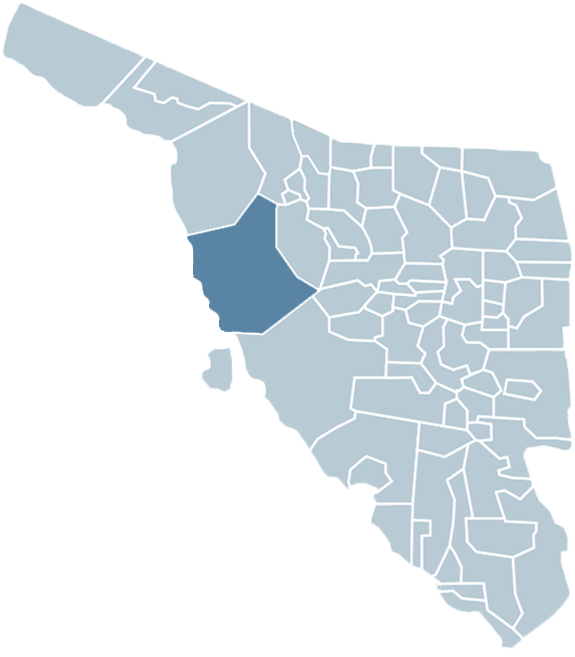
\includegraphics[width=0.25\textwidth]{Pitiquito.png}\\
\caption{\small Figura 1: Pitiquito, Sonora.}
\end{center}
\subsection{Base de Datos.} 
En la base de datos podemos obtener información muy buena sobre los momentos climatológicos que ha pasado el municipio, incluso de ellos podemos observar como han cambiado, si para bien o para mal. Teniendo en cuenta que el cambio climático ha sido de gran influencia durante el paso de los años.\\\\Observando los datos en la base, no hay un gran cambio entre décadas, sin embargo, podemos observar que si se ha realizado un cambio drástico en las temperaturas desde 1962 (que son los datos más completos viejos), con relación al 2015 (que son los datos más actuales). De esto, se puede deducir que el calentamiento global ha influido bastante en las temperaturas máximas y mínimas de la región (y para el mundo en general), teniendo en cuenta que, en el 2015 se lograron en el mes de junio, especificamente el día 19 de junio de 2015, una temperatura máxima de 45°C y que, para esas fechas en el año 1962, era raro y menos frecuente que se llegara a una temperatura tan alta. En base a eso, podemos incluso mirar más a fondo cuantas veces ha ocurrido una temperatura entre 43 a 45 grados en ambos años y ver que en el 2015 se dieron con mucha más frecuencia estas altas temperaturas. \\\\Mientras que, las temperaturas máximas anuales entre ambos años son cada vez más altas, debieramos suponer que esto afecta de la misma manera en el invierno, haciendo que estas épocas del año tambien sean más calidad y claro está, que esto se cumple. En el año 1962, la temperatura mínima máxima (refiriéndonos a la temperatura baja más caliente) que se logró rara vez en invierno llegaba a los 12.5°C. y como es de esperarse, en 2015 estas temperaturas fueron cada vez más frecuentes e incluso se observaban en rangos de 9 a 12.5 grados en días seguidos, viendo que es más frecuente año con año, inviernos más cálidos.
\subsection{Gráficas Climatológicas.} \\

A continuación, vemos en las siguientes gráficas los datos obtenidos por la CONAGUA:
\begin{center}
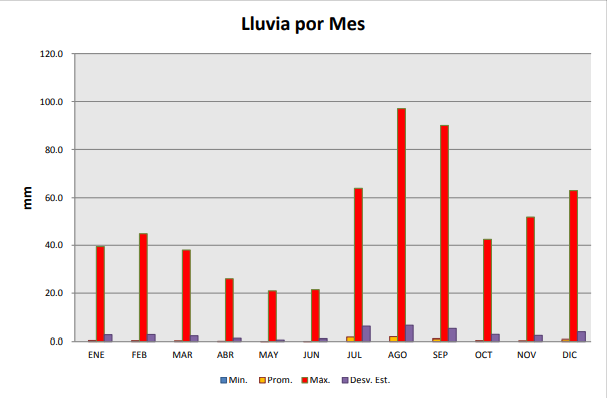
\includegraphics[width=1\textwidth]{Lluvia por mes.png}\\
\caption{\small Figura 2: Lluvia por mes.}\\
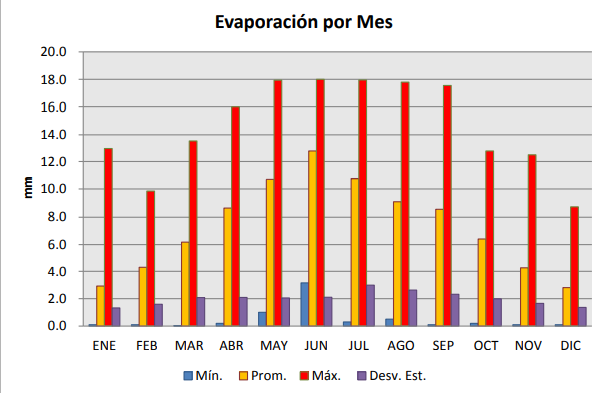
\includegraphics[width=1\textwidth]{Evaporacion por mes.png}\\
\caption{\small Figura 3: Evaporación por mes.}\\
\end{center}  
Debido al promedio, podemos indicar que, en el municipio de Pitiquito, Sonora, las lluvias se frecuentan más en los meses de julio, agosto . Sin embargo, los meses en lo que menos precipitaciones presenta son durante los meses de abril, mayo y junio. 
Tratándo de llegar a un aproximado observado en la Figura 2, las lluvias máximas dadas en el municipio se presentan de 20mm hasta 98mm. Considerando que las lluvias máximas pueden ser influenciadas por alguna tormenta tropical e incluso un huracán aproximado a la región.\\ \\
En la Figura 3, podemos observar como el nivel de evaporación promedio mantiene una figura más o menos simétrica, presentandose las evaporaciones máximas promedio durante los meses intermedio del año, además de esto, podemos observar que, se evaporan en promedio hasta 13mm de agua aproximadamente en el mes de junio, de lo que podemos deducir que, es uno de los meses en los que más calor se ha presentado (lo veremos más adelante).
\begin{center}
\includegraphics[width=1\textwidth]{name/Distribución de la llucia en Rangos de 5mm.png}
\caption{\small Figura 4: Distribución de la lluvia en rangos de 5mm.}
\end{center}
Dentro de esta gráfica, podemos observar que raras veces se lograron lluvias de 100mm, lo que podemos suponer que fue por causas mayores de la naturaleza, como alguna tormenta tropical o un huracán cercano. También podemos darnos cuenta que las lluvias más frecuentes son las menores a 5mm, que se tratan de lluvias leves, que provocan por lo general un aumento en la húmedad caliente en la región (por experiencia propia).
\begin{center}
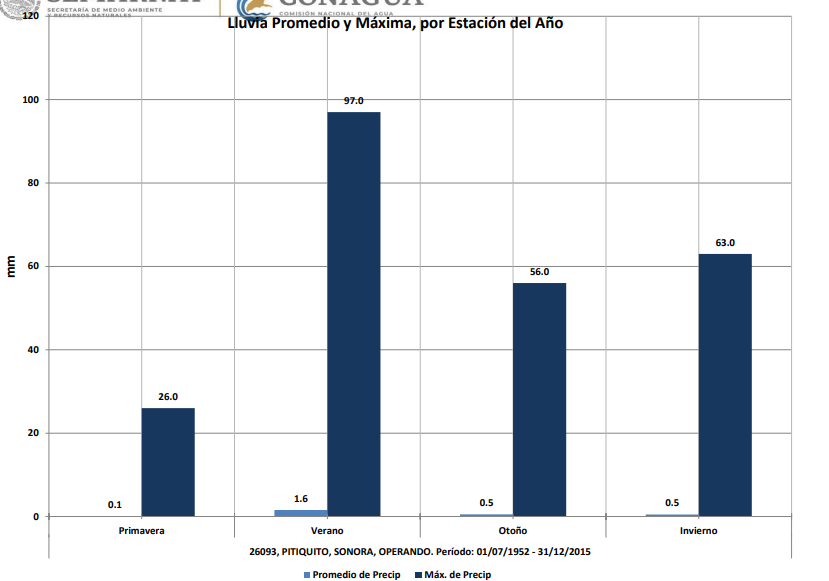
\includegraphics[width=1\textwidth]{name/Lluvia Promedio y Máxima, por Estación del Año.png}
\caption{\small Figura 5: Lluvia promedio y máxima, por estación del año.}
\end{center}
En el municipio se presentan las lluvias más fuertes durante el verano e invierno. Ya lo hemos visto anteriormente, que durante estas fechas también se presentas las precipitaciones más seguidas como las Gemínidas, que son lluvias que todos solemos esperar en fechas navideñas.

\begin{center}
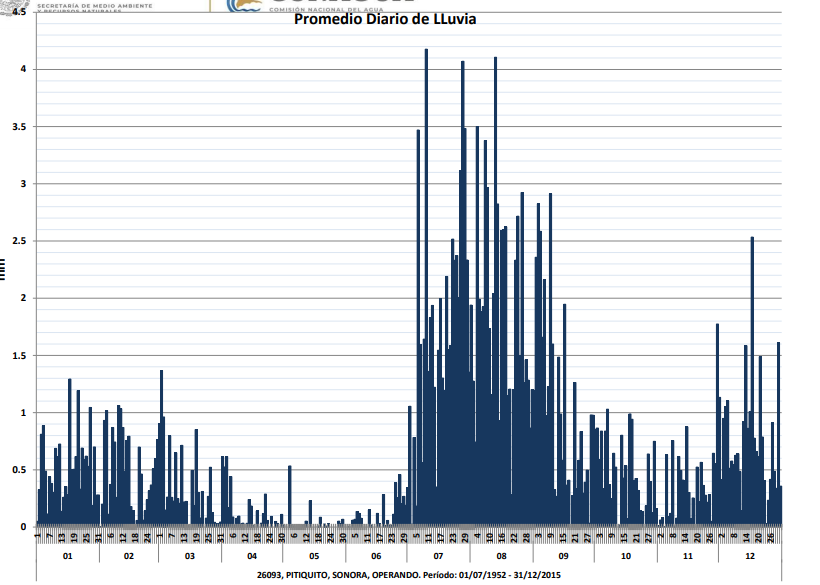
\includegraphics[width=0.90\textwidth]{name/Promedio Diario de Lluvia.png}\\
\caption{\small Figura 6: Promedio Diario de Lluvia.}
\end{center}
Este promedio diario de lluvia nos permite determinar en que días del mes se frecuentan las lluvias más fuertes, para un mejoramiento en cuestiones agrícolas. Dándose a entender que durante los meses de septiembre y octubre se dan las lluvias más abundantes. Sin embargo, con ayuda de los picos altos, podemos ver que durante el mes de diciembre hay precipitaciones fuertes repentinas que han sucedido desde 1952 hasta 2015.
\begin{center}
    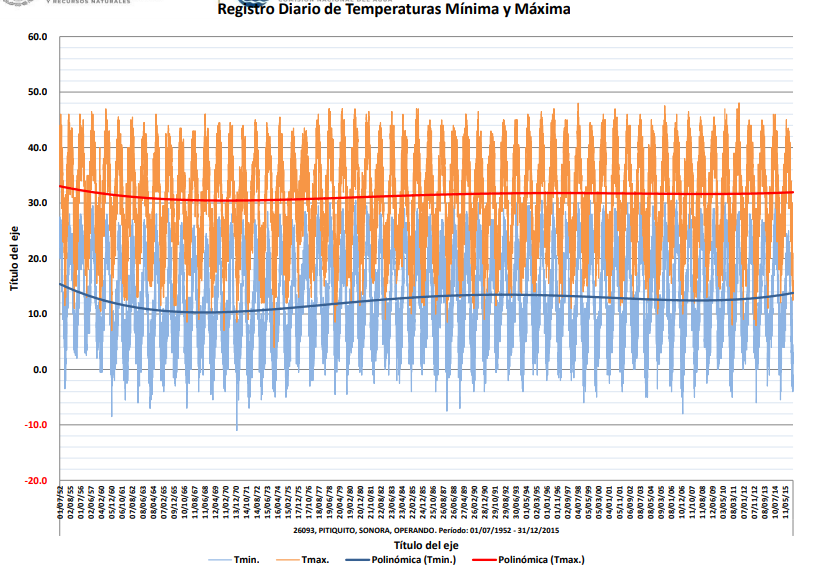
\includegraphics[width=1\textwidth]{name/Registro Diario de Temperaturas Máximas y Mínimas.png}\\
    \caption{\small Figura 7: Resgisto diario temperaturas máximas y mínimas.}
\end{center}
En cuanto a los registros de temperaturas durante el paso de los años, podemos observar que, al inicio del promedio se logra apreciar un promedio más alto, pero es por la falta de datos de los primeros años. Tomaremos en cuenta el promedio mínimo (aproximadamente por 1967) hasta la actualidad. De este promedio se observa que, el promedio cada vez es más alto, notando que una vez el promedio sube, ya no vuelve a recuperar el valor anterior. Retomando una vez más, que con el paso de los años, las temperaturas máximas son cada vez más frecuentes gracias al calentamiento global.\\\\Por otra parte, de igual manera, la temperatura mínima promedio va aumentando, dandonos cuenta que, las temperaturas bajas cada vez son más calientes (aunque suene raro decirlo).
\begin{center}
    \includegraphics[width=1\textwidth]{name/Temperatura Máxima.png}
    \caption{\small Figura 8: Temperaturas máximas.}
    \includegraphics[width=1\textwidth]{name/Temperatura Mínima.png}
    \caption{\small Figura 9: Temperaturas mínimas.}
    
\end{center}
En las gráficas de temperaturas podemos observar como la región municipal de Pitiquito, Sonora. Presenta temperaturas muy cálidas debido a que, la mayor parte del año, la temperatura mínima ronda sobre los 30 grados. llegando en verano a temperaturas incluso mayores a 45 grados (hablando del promedio).\\\\Como última gráfica, veremos algo que abarque ambos rasgos:
\begin{center}
    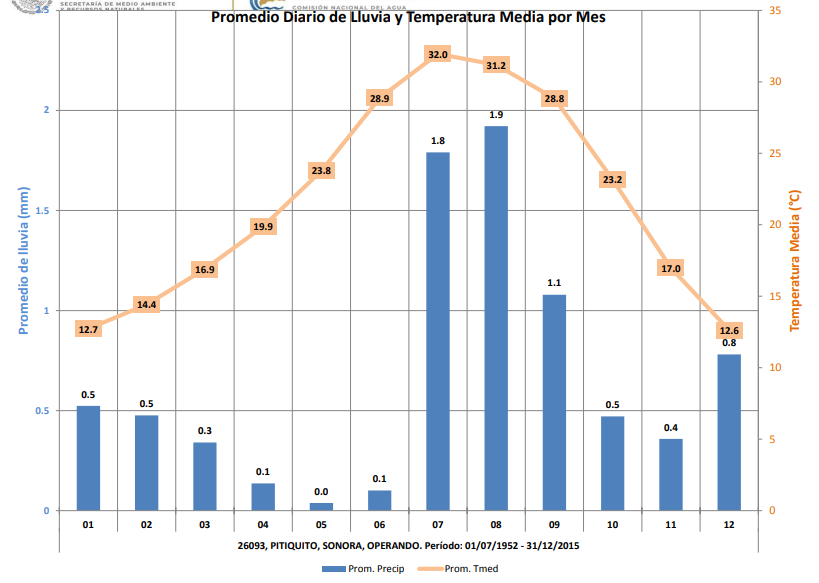
\includegraphics[width=1\textwidth]{name/Promedio Diario de Lluvia y Temperatura Media por Mes.png}\\
    \caption{\small Figura 10: Promedio Diario de Lluvia y Temperatura Media por Mes.}\\
\end{center}
Debido a que el sitio que analizamos es un deierto, por lo general la evaporación de agua provoca aumentos en la temperatura cuando se presentan en los meses de verano. Como podemos admirar en la gráfica, cuando se dan las precipitaciones altas, por lo general, se observa un aumento promedio de la temperatura de igual manera, por ello es que en el municipio no dura tanto tiempo húmedo, suelen secarse los alrededores en cuestiones de días. Claro está, que las temperaturas al aumentar, se hacen demasiadas intensas. 
\maketitle
\section{Conclusión.}
El cambio climático es algo con lo que estamos cada vez más concienciados. Conforme pasan los años, avanzan las tecnologías van produciendo un gran impacto en cada región del mundo. Durante este documento, nos podemos dar cuenta como ha afectado a lo largo de los últimos 63 años en el municipio de Pitiquito. Podemos ser observadores y juzgar como ha afectado el calentamiento global en nuestros alrededores, teniendo como base, estos datos publicados y calculados por las administraciones de nuestro país.\\\\De forma más individual puedo decir que, la realización de esta actividad me ayudó de muy buena manera, para poder entender la realización de textos en Overleaf. También para fomentar la práctica del mismo y poder observar el cambio de nuestros alrededores a lo largo de los años.\\Por otro lado, habrá que mejorar el método de escritura porque, durante el trabajo, se me dificultó mucho encontrar diferentes maneras de expesar mis palabras para que no sonara repetitivo.
\maketitle
\section{Referencias.}
\begin{enumerate}
    \item https://smn.conagua.gob.mx/es/climatologia/informacion-climatologica/informacion-estadistica-climatologica
    \item https://www.overleaf.com/learn
\end{enumerate}
\end{document}
